\documentclass{article}\usepackage{graphicx, color}
%% maxwidth is the original width if it is less than linewidth
%% otherwise use linewidth (to make sure the graphics do not exceed the margin)
\makeatletter
\def\maxwidth{ %
  \ifdim\Gin@nat@width>\linewidth
    \linewidth
  \else
    \Gin@nat@width
  \fi
}
\makeatother

\IfFileExists{upquote.sty}{\usepackage{upquote}}{}
\definecolor{fgcolor}{rgb}{0.2, 0.2, 0.2}
\newcommand{\hlnumber}[1]{\textcolor[rgb]{0,0,0}{#1}}%
\newcommand{\hlfunctioncall}[1]{\textcolor[rgb]{0.501960784313725,0,0.329411764705882}{\textbf{#1}}}%
\newcommand{\hlstring}[1]{\textcolor[rgb]{0.6,0.6,1}{#1}}%
\newcommand{\hlkeyword}[1]{\textcolor[rgb]{0,0,0}{\textbf{#1}}}%
\newcommand{\hlargument}[1]{\textcolor[rgb]{0.690196078431373,0.250980392156863,0.0196078431372549}{#1}}%
\newcommand{\hlcomment}[1]{\textcolor[rgb]{0.180392156862745,0.6,0.341176470588235}{#1}}%
\newcommand{\hlroxygencomment}[1]{\textcolor[rgb]{0.43921568627451,0.47843137254902,0.701960784313725}{#1}}%
\newcommand{\hlformalargs}[1]{\textcolor[rgb]{0.690196078431373,0.250980392156863,0.0196078431372549}{#1}}%
\newcommand{\hleqformalargs}[1]{\textcolor[rgb]{0.690196078431373,0.250980392156863,0.0196078431372549}{#1}}%
\newcommand{\hlassignement}[1]{\textcolor[rgb]{0,0,0}{\textbf{#1}}}%
\newcommand{\hlpackage}[1]{\textcolor[rgb]{0.588235294117647,0.709803921568627,0.145098039215686}{#1}}%
\newcommand{\hlslot}[1]{\textit{#1}}%
\newcommand{\hlsymbol}[1]{\textcolor[rgb]{0,0,0}{#1}}%
\newcommand{\hlprompt}[1]{\textcolor[rgb]{0.2,0.2,0.2}{#1}}%

\usepackage{framed}
\makeatletter
\newenvironment{kframe}{%
 \def\at@end@of@kframe{}%
 \ifinner\ifhmode%
  \def\at@end@of@kframe{\end{minipage}}%
  \begin{minipage}{\columnwidth}%
 \fi\fi%
 \def\FrameCommand##1{\hskip\@totalleftmargin \hskip-\fboxsep
 \colorbox{shadecolor}{##1}\hskip-\fboxsep
     % There is no \\@totalrightmargin, so:
     \hskip-\linewidth \hskip-\@totalleftmargin \hskip\columnwidth}%
 \MakeFramed {\advance\hsize-\width
   \@totalleftmargin\z@ \linewidth\hsize
   \@setminipage}}%
 {\par\unskip\endMakeFramed%
 \at@end@of@kframe}
\makeatother

\definecolor{shadecolor}{rgb}{.97, .97, .97}
\definecolor{messagecolor}{rgb}{0, 0, 0}
\definecolor{warningcolor}{rgb}{1, 0, 1}
\definecolor{errorcolor}{rgb}{1, 0, 0}
\newenvironment{knitrout}{}{} % an empty environment to be redefined in TeX

\usepackage{alltt}
\title{Mixed GWR Simulation Write-up}
\author{Aaron Swoboda}


\begin{document}
\maketitle

What are our research questions? Basically:
\begin{enumerate}
\item Can we find the ``true'' model among the eight different possibilities with three model parameters?
\item Are there differences in the results based on the metric used?
\item What happens as we change the sample size and amount of error in the model?
\item How much does it really matter if we are concerned with coefficient estimates?
\item What happens when we use other decision tools to help with model selection? (Monte Carlo simulations and test statistics)
\end{enumerate}





\section{Methodology}

Imagine a simple linear model with two explanatory variables,
\begin{equation}
Y = \beta _0 + \beta _1 *X_1 + \beta _2 * X_2 + \epsilon
\end{equation}
Now imagine that each of our $N$ individual observations in this model occur at geographical locations on a Cartesian plane. Thus our data consists of an $N x 5$ matrix, where $Y$ may be house prices, $X_1$ and $X_2$ could be the living space and lot size associated with each house, and the final two columns determine the location of the observations (for instance, latitude and longitude, or distances north and east from a prescribed point serving as the origin).

The above simple model exemplifies spatial stationarity in the parameters. The $\beta$ coefficients are constant over space. Instead, the coefficients could exhibit spatial non-stationarity, in which case one, two, or all three of the $\beta$ coefficients are a function of location. This has a natural interpretation in the current real estate example. Location matters. Location can matter in different ways. For instance, if the value of land varies over space, then we would expect the coefficient on lot size to vary over space, while it is also possible that the intercept varies over space to reflect variation in prices of similar houses in different locations. 

While it is possible to parameterize the variation in coefficients, for instance researchers often (CITATION?) include a variable measuring the distance from an observation to an important amenity such as the Central Business District and then this distance variable could be interacted with variables whose value are predicted to vary over space. However, it is not implausible to believe that the variation in coefficients might not be easily parameterized (for instance, if land values are a non-monotonic function of distance). Researchers may instead interact variables with fixed effects for cities or census tracts. However, such strategies require the analyst to make assumptions that severely limit the type and degree of variation in the parameters. For instance, interaction terms with geographic boundaries assume discrete differences in the value of parameters across the boundaries, while instead the parameters may instead be a continuous function of location.

\subsection{Local Regression to the Rescue?}


\subsection{Experimental Design}

We generate data in the following format:
\begin{equation}
Y = \beta _0(location) + \beta _1(location) *X_1 + \beta _2(location) * X_2 + \epsilon ,
\end{equation}
where sometimes the coefficient is in fact stationary, $\beta _i(location) = \beta$, and other times it is non-stationary. With three coefficients each having the possibility of being stationary or not, there are eight different possible combinations, ranging from (stationary, stationary, stationary) to (non-stationary, non-stationary, non-stationary).

We generate data using all eight different combinations and then estimate all eight possible LWR models (assuming non-stationarity or not for each variable). We then calculate different Cross-Validation metrics and compare their values across models and bandwidths. 

We have three different values for each coefficient in our DGP, no variation, some variation, and more variation.

We also change the sample size of our data as well as the variance of the model error term.

\section{Simulation Results}

We have seven different ways to pick the ``best'' model (the AIC, GCV, SCV, LOOCV, and RMSEs for the three different coefficients). Here are tables showing the relative frequency (in percentage) that each model number was selected by optimizing a given metric. Note that the columns in the following tables may not sum exactly to 100 due to rounding.




\begin{knitrout}
\definecolor{shadecolor}{rgb}{0.969, 0.969, 0.969}\color{fgcolor}\begin{kframe}
\begin{alltt}
\hlfunctioncall{for} (i in 1:8) \{
    temp2 = \hlfunctioncall{which}(mcOutput[, \hlstring{"True Model"}, ] == i, arr.ind = TRUE)
    temp3 = mcOutput[8:14, \hlstring{"Model Number"}, \hlfunctioncall{unique}(temp2[, 2])]
    temp4 = \hlfunctioncall{factor}(temp3)
    
    newdata = \hlfunctioncall{data.frame}(ModelNum = temp4, Metric = \hlfunctioncall{factor}(\hlfunctioncall{rownames}(temp3), 
        levels = \hlfunctioncall{rownames}(temp3)))
    \hlfunctioncall{cat}(\hlfunctioncall{paste}(\hlstring{"\textbackslash{}n true model ="}, i, \hlstring{"\textbackslash{}n"}))
    \hlfunctioncall{cat}(\hlstring{"spatial variation...\textbackslash{}n"})
    \hlfunctioncall{print}(models[i, ])
    \hlfunctioncall{print}(\hlfunctioncall{round}(\hlfunctioncall{table}(newdata) * 100 * 7/\hlfunctioncall{sum}(\hlfunctioncall{table}(newdata)), 0))
\}
\end{alltt}
\begin{verbatim}
## 
##  true model = 1 
## spatial variation...
##   beta0 beta1 beta2
## 1    no    no    no
##         Metric
## ModelNum AIC GCV SCV LOOCV B0RMSE B1RMSE B2RMSE
##        1   0   0   0    75      6      7      6
##        2  26  26   0     6      5     22     20
##        3  34  33   0     6     21      4     22
##        4   1   1   8     2      5      3     37
##        5  38  38   0     7     20     21      4
##        6   1   1   8     2      5     35      3
##        7   1   1   5     1     32      4      5
##        8   0   0  78     0      5      3      2
## 
##  true model = 2 
## spatial variation...
##   beta0 beta1 beta2
## 2   yes    no    no
##         Metric
## ModelNum AIC GCV SCV LOOCV B0RMSE B1RMSE B2RMSE
##        1   0   0   0     4      0      4      4
##        2  91  91  37    89     94     29     29
##        3   4   4   0     2      1      6     25
##        4   0   1  16     1      1      1     32
##        5   4   4   0     3      1     24      6
##        6   0   1  16     1      1     33      1
##        7   0   0   3     0      1      2      2
##        8   0   0  28     0      0      1      1
## 
##  true model = 3 
## spatial variation...
##   beta0 beta1 beta2
## 3    no   yes    no
##         Metric
## ModelNum AIC GCV SCV LOOCV B0RMSE B1RMSE B2RMSE
##        1   0   0   0    12     13      0     13
##        2  11  11   1     7      1      2     24
##        3  77  76   0    65     23     66     22
##        4   2   2  12     4      4      6     32
##        5   8   8   0     5     24      2      1
##        6   0   0   9     1      2      3      2
##        7   2   2   6     5     29     15      3
##        8   0   0  72     1      4      6      2
## 
##  true model = 4 
## spatial variation...
##   beta0 beta1 beta2
## 4   yes   yes    no
##         Metric
## ModelNum AIC GCV SCV LOOCV B0RMSE B1RMSE B2RMSE
##        1   0   0   0     2      1      0      6
##        2  70  68  29    65     65      6     29
##        3  10   9   0     8      2     34     25
##        4  16  19  25    21     25     14     34
##        5   2   2   0     2      2      4      2
##        6   0   1  13     1      2      8      1
##        7   0   0   3     1      2     22      2
##        8   0   0  30     0      2     12      1
## 
##  true model = 5 
## spatial variation...
##   beta0 beta1 beta2
## 5    no    no   yes
##         Metric
## ModelNum AIC GCV SCV LOOCV B0RMSE B1RMSE B2RMSE
##        1   0   0   0    12     13     13      0
##        2  11  10   1     7      1     24      2
##        3   8   8   0     4     24      1      2
##        4   0   1   9     1      1      2      3
##        5  78  77   0    66     23     23     66
##        6   1   2  12     5      5     32      6
##        7   1   2   6     4     30      3     15
##        8   0   0  73     1      4      2      6
## 
##  true model = 6 
## spatial variation...
##   beta0 beta1 beta2
## 6   yes    no   yes
##         Metric
## ModelNum AIC GCV SCV LOOCV B0RMSE B1RMSE B2RMSE
##        1   0   0   0     2      1      6      0
##        2  71  68  29    66     65     30      7
##        3   3   2   0     2      2      2      4
##        4   0   0  13     1      2      1      7
##        5  10   9   0     8      2     24     34
##        6  16  19  24    20     25     33     14
##        7   0   1   3     1      2      2     21
##        8   0   0  30     0      2      1     13
## 
##  true model = 7 
## spatial variation...
##   beta0 beta1 beta2
## 7    no   yes   yes
##         Metric
## ModelNum AIC GCV SCV LOOCV B0RMSE B1RMSE B2RMSE
##        1   0   0   0     5     13      1      1
##        2   8   8   1     6      0      2      2
##        3  25  24   0    18     25     16      2
##        4   1   2   9     3      1     12      4
##        5  25  24   0    18     25      2     17
##        6   2   2   9     3      1      5     12
##        7  39  40   8    44     31     50     51
##        8   1   1  72     3      4     11     11
## 
##  true model = 8 
## spatial variation...
##   beta0 beta1 beta2
## 8   yes   yes   yes
##         Metric
## ModelNum AIC GCV SCV LOOCV B0RMSE B1RMSE B2RMSE
##        1   0   0   0     1      1      1      1
##        2  60  57  23    53     48      7      7
##        3   6   5   0     5      3     15      5
##        4   9  11  19    12     14     16      8
##        5   6   5   0     5      3      5     16
##        6   9  11  19    11     14      8     15
##        7   3   3   3     4      4     32     33
##        8   6   7  35     8     14     16     15
\end{verbatim}
\end{kframe}
\end{knitrout}


The results of the previous tables must be taken with a grain of salt, as there are frequently times when a ``true'' model may include variation in a coefficient, but the degree of non-stationarity in the coefficient may be small. In such cases, choosing an incorrect model (such as one that keeps such a coefficient constant) may not be such a big problem. 

Some patterns clearly emerge. 
\begin{itemize}
\item The AIC and GCV metrics \emph{never} select Model 1, even when it is the actual model.
\item There are several occasions where the model/bandwidth combination with the smallest RMSE is not the ``correct'' model.
\end{itemize}

\subsection{Coefficient Formulation}

Even if an incorrect model is chosen, the model may yield accurate estimates of the coefficients. In each run of the simulation we estimated 50 different model/bandwidth combinations (seven different bandwidths for each of the seven models with at least one coefficient varying over space, plus the standard OLS model). We calculate the Root Mean Squared Error for each model and can rank these values. For instance, it is possible, and often the case, that the ``wrong'' model yields the most accurate estimates of a coefficient.

\begin{knitrout}
\definecolor{shadecolor}{rgb}{0.969, 0.969, 0.969}\color{fgcolor}\begin{kframe}
\begin{alltt}
\hlcomment{# \hlfunctioncall{for} (i in 1:8) \{}
i = 1
temp2 = \hlfunctioncall{which}(mcOutput[1, \hlstring{"True Model"}, ] == i)
inputMetrics = \hlfunctioncall{c}(\hlstring{"AIC"}, \hlstring{"GCV"}, \hlstring{"SCV"}, \hlstring{"LOOCV"})
inputStats = \hlfunctioncall{c}(\hlstring{"B0RMSE Rank"}, \hlstring{"B1RMSE Rank"}, \hlstring{"B2RMSE Rank"})
\hlfunctioncall{par}(mfrow = \hlfunctioncall{c}(4, 3))
\hlfunctioncall{for} (j in 1:4) \{
    \hlfunctioncall{for} (k in 1:3) \{
        temp3 = mcOutput[inputMetrics[j], inputStats[k], temp2]
        \hlcomment{# \hlfunctioncall{summary}(temp3)}
        \hlfunctioncall{hist}(temp3, xlim = \hlfunctioncall{c}(0, 50), breaks = 5 * (0:10), col = \hlstring{"grey85"}, axes = F, 
            ylab = \hlstring{"rel freq"}, xlab = \hlstring{"rank"}, main = \hlstring{""})
    \}
\}
\end{alltt}
\end{kframe}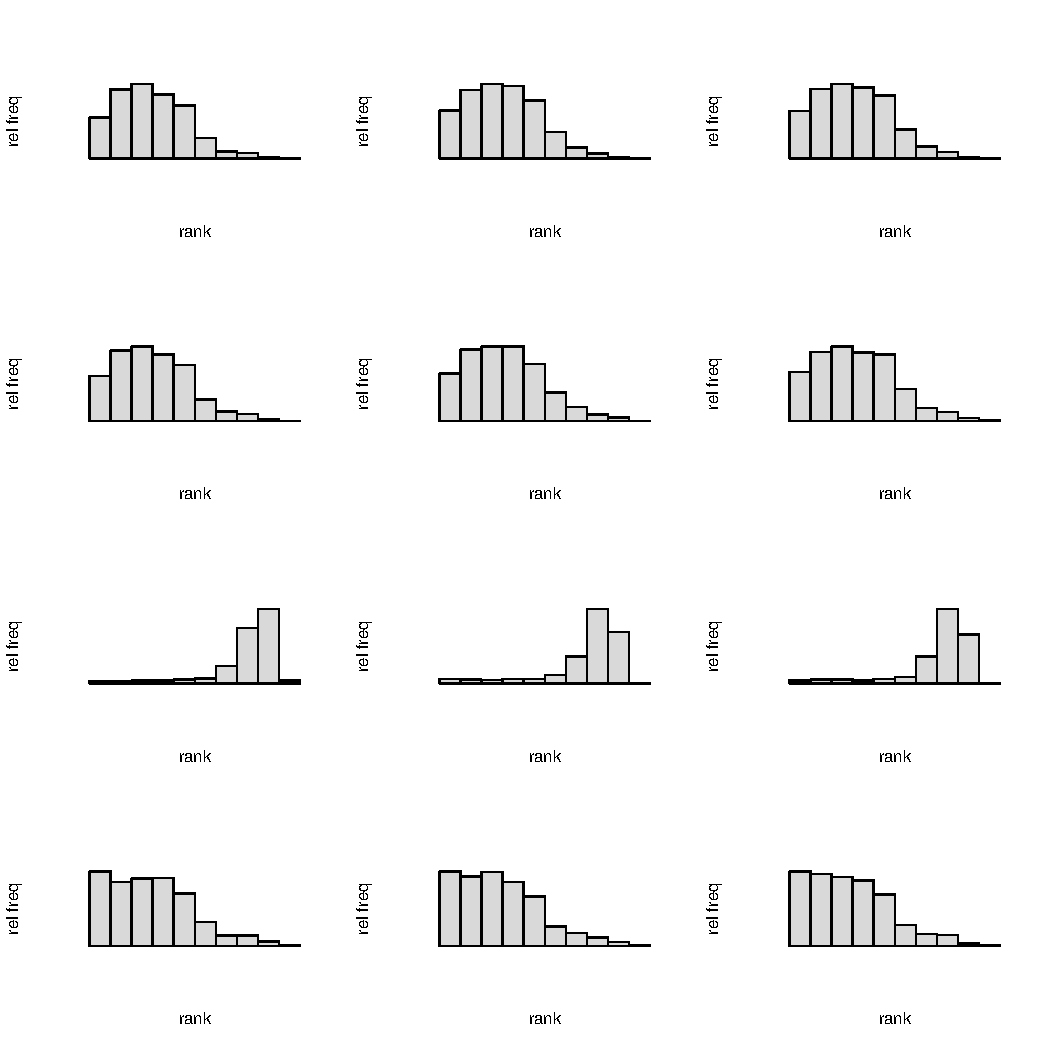
\includegraphics[width=\maxwidth]{figure/BetaRankTabulations} \begin{kframe}\begin{alltt}
\hlcomment{# \}}
\end{alltt}
\end{kframe}
\end{knitrout}

\end{document}
